\documentclass[a4paper,12pt]{article} 

\usepackage{blindtext}
\usepackage{titlesec}
\usepackage{amsmath,amsthm,amsfonts,amssymb,mathrsfs}
\usepackage{graphicx}
\usepackage[english]{babel}
\usepackage[section]{placeins}
\usepackage{float}
\usepackage{physics}
\usepackage{subfig}

\addtolength{\topmargin}{-.875in}
\addtolength{\textheight}{1.75in}

\begin{document}
\begin{titlepage}
    \begin{center}
        \vspace*{1cm}
        \Huge
        \textbf{Final Project}
        
        \Large
        \vspace{2.5cm}
        \textbf{Martin Waites\\ Peicen Liu\\ Yichen Liu\\ Alexander Knyazev}
        \vspace{3.5cm}
        \begin{center}
           
\includegraphics[height=7.7cm]
           {LU_logo.png}
        \end{center}
        \vfill
        \vspace{0.8cm}
        \Large
        MNXB01 - Introduction to Programming and Computing for Scientists\\
        Lund University\\
        November 2019
    \end{center}
\end{titlepage}

\newpage


\section{Introduction}

The purpose of the project is to demonstrate some of the things we have learned about data processing and analysis throughout the course. To this end we have been given data about temperatures measured in different locations around Sweden. This data comes from the Swedish Meteorological and Hydrological Institute (SMHI) where in some cases measurements have been going on for hundreds of years. From this data we produced five different types of results named oneDay, WarmColdDay, everyDay, LattDiff and getTemperature named after the names of the main functions called to produce the results.\\\\



\section{Function Descriptions}

\subsection{Data Cleaning}
\paragraph{}
The raw data files were in the CSV form. Some small manual modifications were done first, such as taking away the description lines at the beginning of the files, and the rest cleaning process was done by a Python function. The input arguments of the function are the directory of where the original data file and the directory to store the clean data file. The function converts the CSV file into a .dat file which has the format [year, month, day, temperature] in each line. Some of the subsequent analysis functions are created for the clean data files.


\subsection{oneDay}
\paragraph{}
The oneDay function is consisted of three parts, or three sub-functions. The first part is called oneDayMDI which takes two integers (month and date) as inputs and outputs either a histogram showing the temperature of the input day in every year, or an array that contains the mean and the standard deviation of the input day. The output is decided by the argument plot=0 for producing the array and plot=1 for generating the histogram. The second part is called oneDay and takes one input argument of the day number (an integer between 1 and 365). The output is the same as in part one. However, it was decided to skip the 29th of February in each leap year for the second part, and therefore the day number only goes up to 365. An example histogram is shown in Figure \ref{fig:oneDayMDI_uppsala}, and it shows the temperature on the Christmas day in Uppsala from 1722 to 2013. 
\begin{figure}[h!]
    \centering
    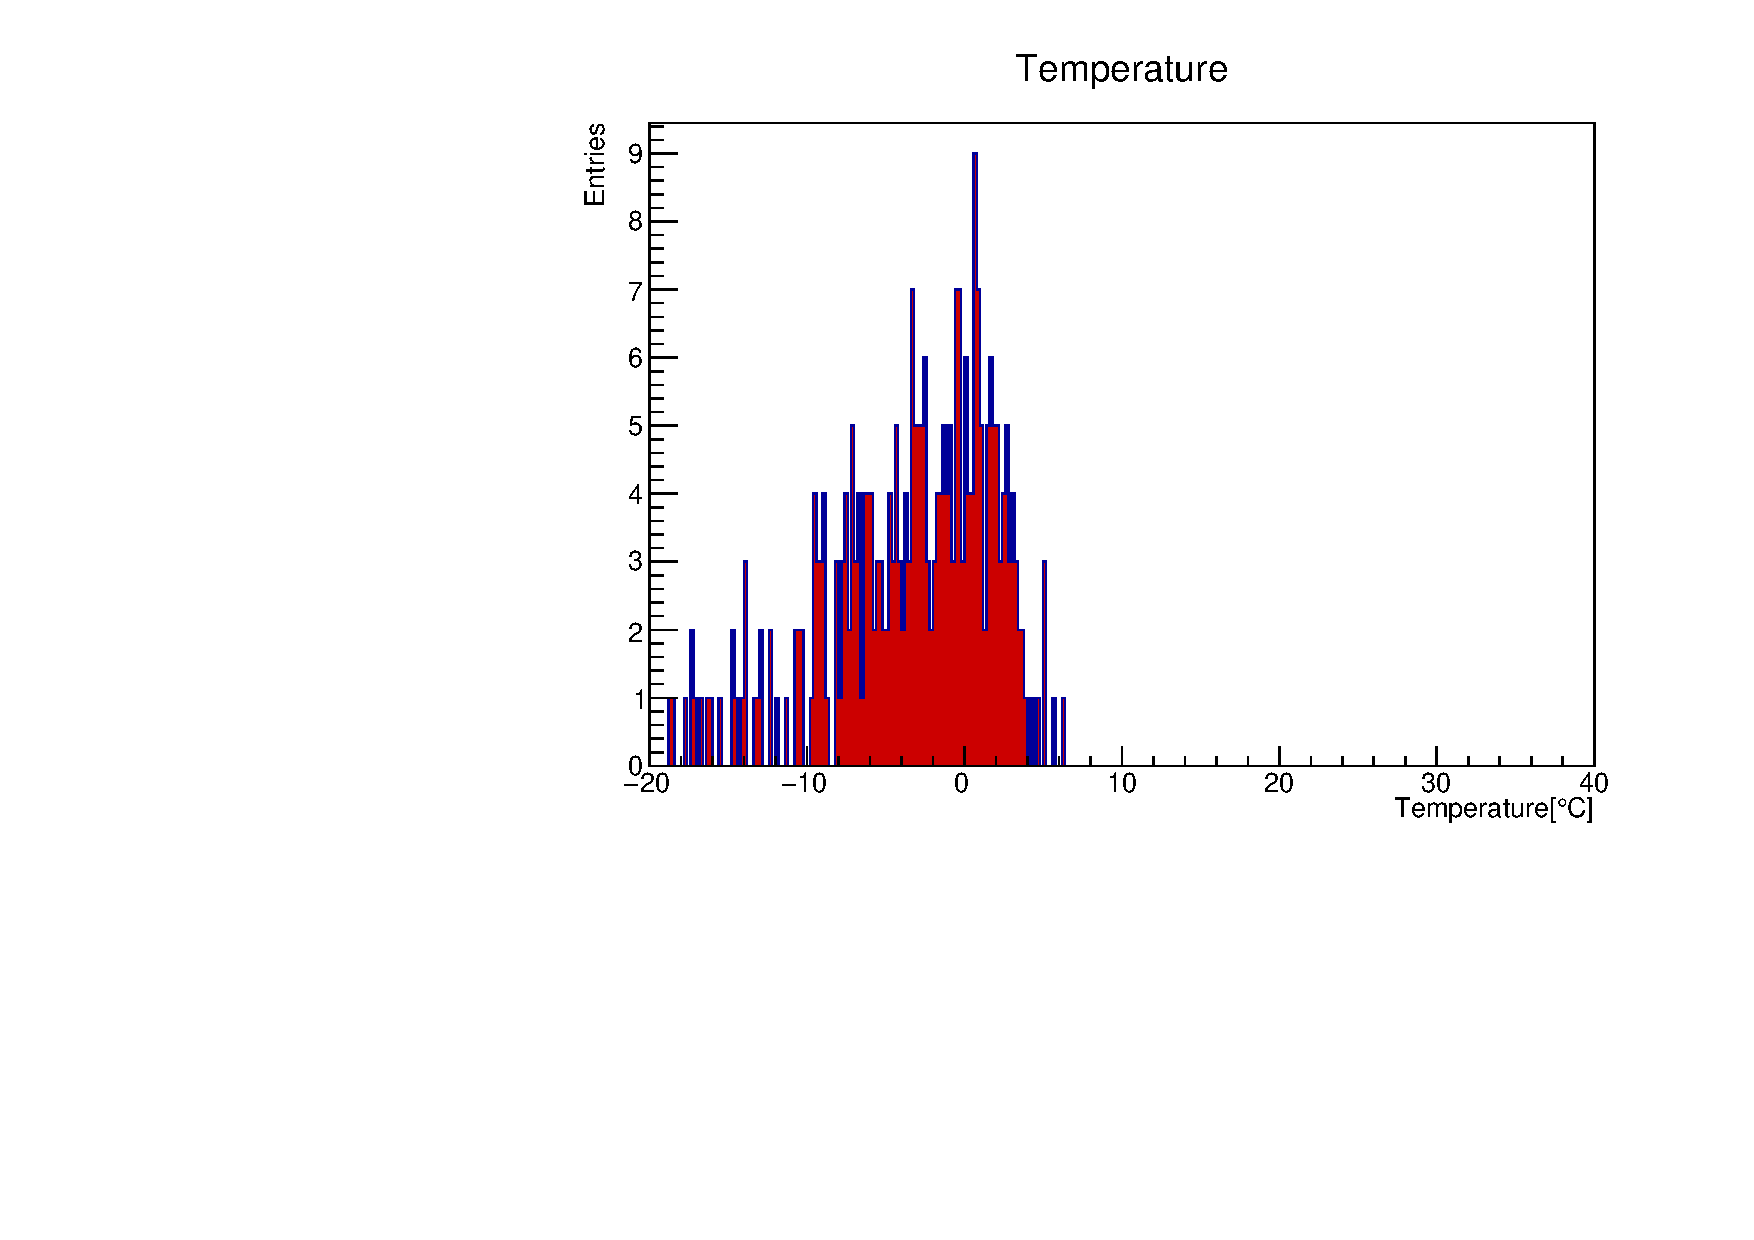
\includegraphics[scale = 0.8]{oneDayMDI_uppsala.pdf}
    \caption{Christmas day temperature in Uppsala from 1722 to 2013}
    \label{fig:oneDayMDI_uppsala}
\end{figure}
\paragraph{}
The third part is different from the previous two parts. The function for the third part is called oneDayProb which takes input arguments of month, day, a given temperature and an error range. The function computes the probability of getting the given temperature, for a specific date in a region, within plus/minus half of the given error range. The function uses Gaussian distribution for the probabilistic modelling which is the most reasonable distribution in this case. For example, oneDayProb("uppsala.dat", 12, 25, -1, 2) calculates the probability of getting a temperature between -2 and 0 (-1 plus/minus 1) on the Christmas day in Uppsala. 





\subsection{WarmColdDay}

The WarmColdDay function demonstrates the days of warmest and coldest days occurred at and the output shown by histogram allows us to visualise when the warmest and coldest days are most likely to occur during the year. A Gaussian function is plotted to the histogram to fit the distribution.\\

Figure \ref{fig:WarmCold} shows the output of this function, where the blue and red histogram indicates the coldest and warmest days respectively, while the blue and red gaussian line indicates the distribution of warmest and coldest days respectively. 







\begin{figure}[h!]
    \centering
    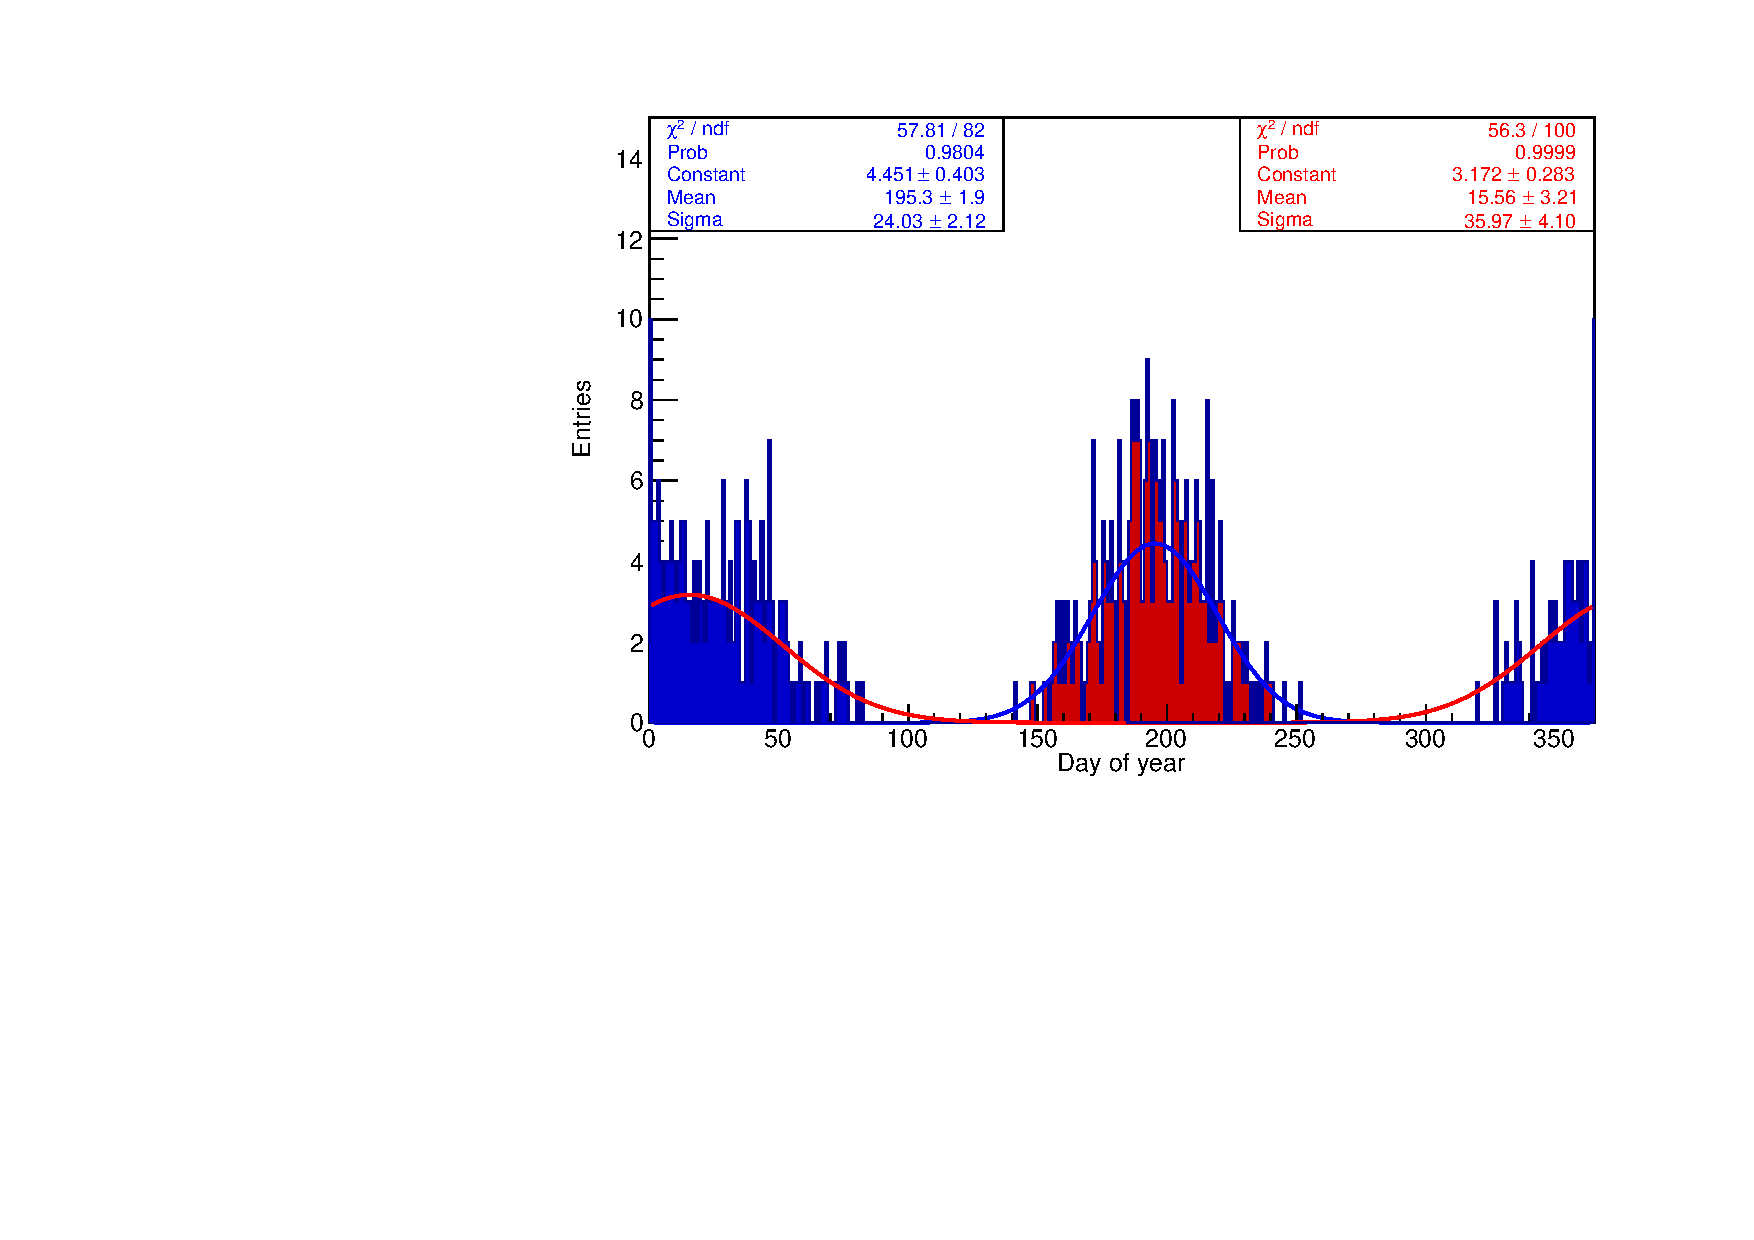
\includegraphics[scale = 0.8]{uppsala.pdf}
    \caption{Warmest and coldest day in Uppsala}
    \label{fig:WarmCold}
\end{figure}


\begin{table}[h!]
    \centering
    \begin{tabular}{l l l l l}
    \hline
    Location     & \multicolumn{2}{c}{Mean Value}     
             & \multicolumn{2}{c}{Standard Deviation}\\
    \hline
             & Cold           & Warm          & Cold           & Warm  \\

    Uppsala  & $15.6\pm3.2$ & $195.3\pm1.9$ & $36.0\pm4.1$ & $24.0\pm2.1$\\
    
    Luleå    & $20\pm28$   & $178\pm50$   & $71\pm54$      & $80\pm149$ \\
    
    Umeå     & $23\pm44$   & $187\pm91$   & $82\pm95$      & $122\pm143$ \\
    
    Visby    & $29\pm55$   & $211\pm73$   & $144\pm212$    & $92\pm166$ \\
    
    Lund     & $25\pm60$   & $184\pm8$    & $105\pm188$    & $81\pm84$ \\
    \hline
    \end{tabular}
    \caption{Mean Value and Standard Deviation }
    \label{tab:WarmCold_Table}
\end{table}




\subsection{everyDay and LattDiff}

The everyDay function produces a plot showing the mean and standard deviation of the temperature of each day for every day of the year. This allows us to visualise how the temperature changes over the year and see when the seasons occur. Figure \ref{fig:everyDay} shows the output of this function.\\

\begin{figure}[h!]
    \centering
    
\includegraphics[scale = 0.7]{every_day_graph_one_location_histogram.pdf}
    \caption{histogram plot produced by the everyDay function}
    \label{fig:everyDay}
\end{figure}


The LattDiff function produces two plots, these plots show the temperature of each day for every day of the year similarly to the everyDay function however for five locations of different Latitudes. This allows us to  
show the effect of latitude on the temperature distribution over the year. Figure \ref{fig:LattDiff} shows this graph while Figure \ref{fig:LattDiff_no} in the Results shows only the mean without the standard deviation in order to get a clearer image of the change with Latitude.

\begin{figure}[h!]
    \centering
    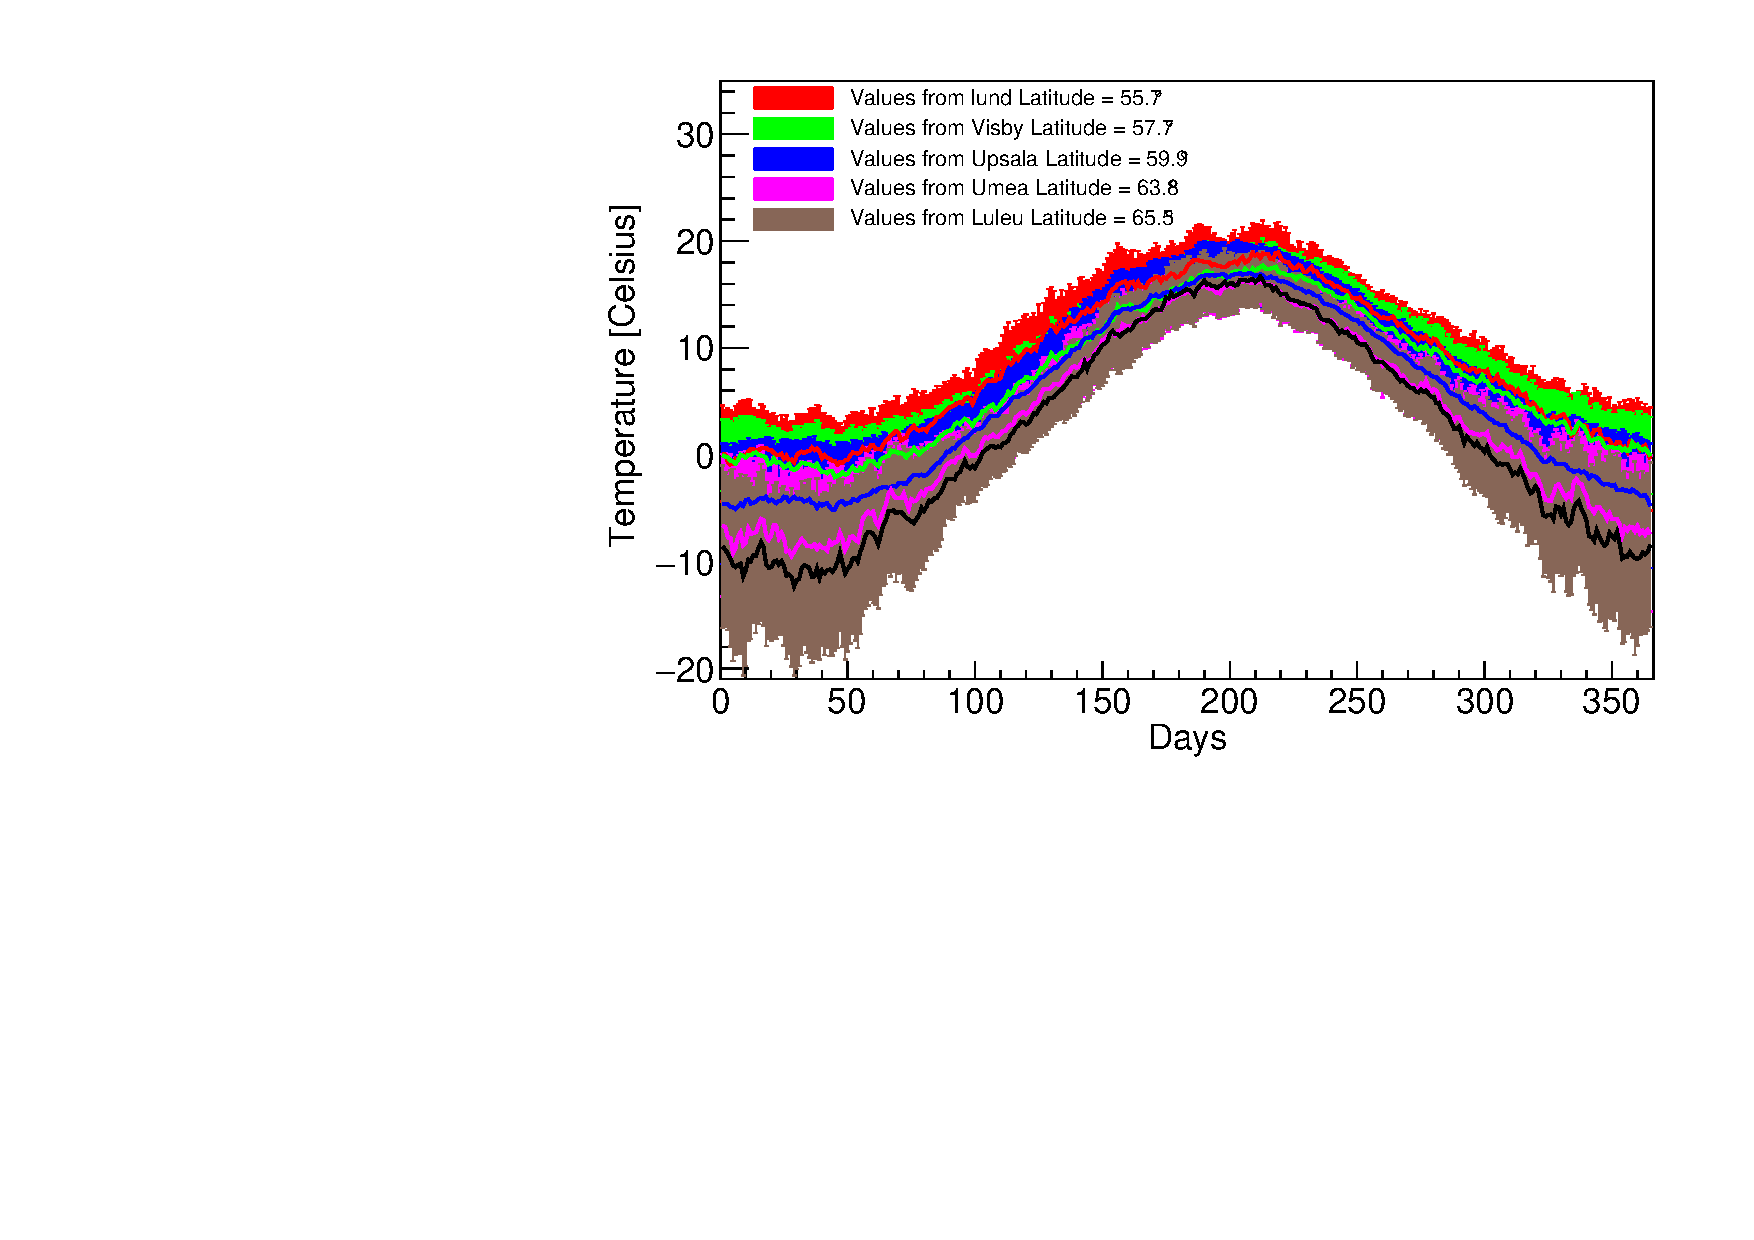
\includegraphics[scale = 0.7]{every_day_graph_multiple_locations_standard_deviations_included.pdf}
    \caption{Plot produced by the LattDiff function}
    \label{fig:LattDiff}
\end{figure}







\subsection{getTemperature}

The \texttt{getTemperature} function reads an initial data file for a location from 
a predefined list, which includes Boras, Falsterbo, Falun, Karlstad, Lulea, Lund,
Soderarm, Umea, Uppsala and Visby. The function plots the data and makes a linear fit 
of the data, and save result as a \texttt{.pdf} document. The time axis on the plot
is in seconds, to include the leap years. The fit results can be interpreted as 
the average temperature in the location (\texttt{p0}) in $^\circ$C and the change of
average temperature over time (\texttt{p1}) in $^\circ$C/s. 

\begin{figure}
    \centering
    \subfloat{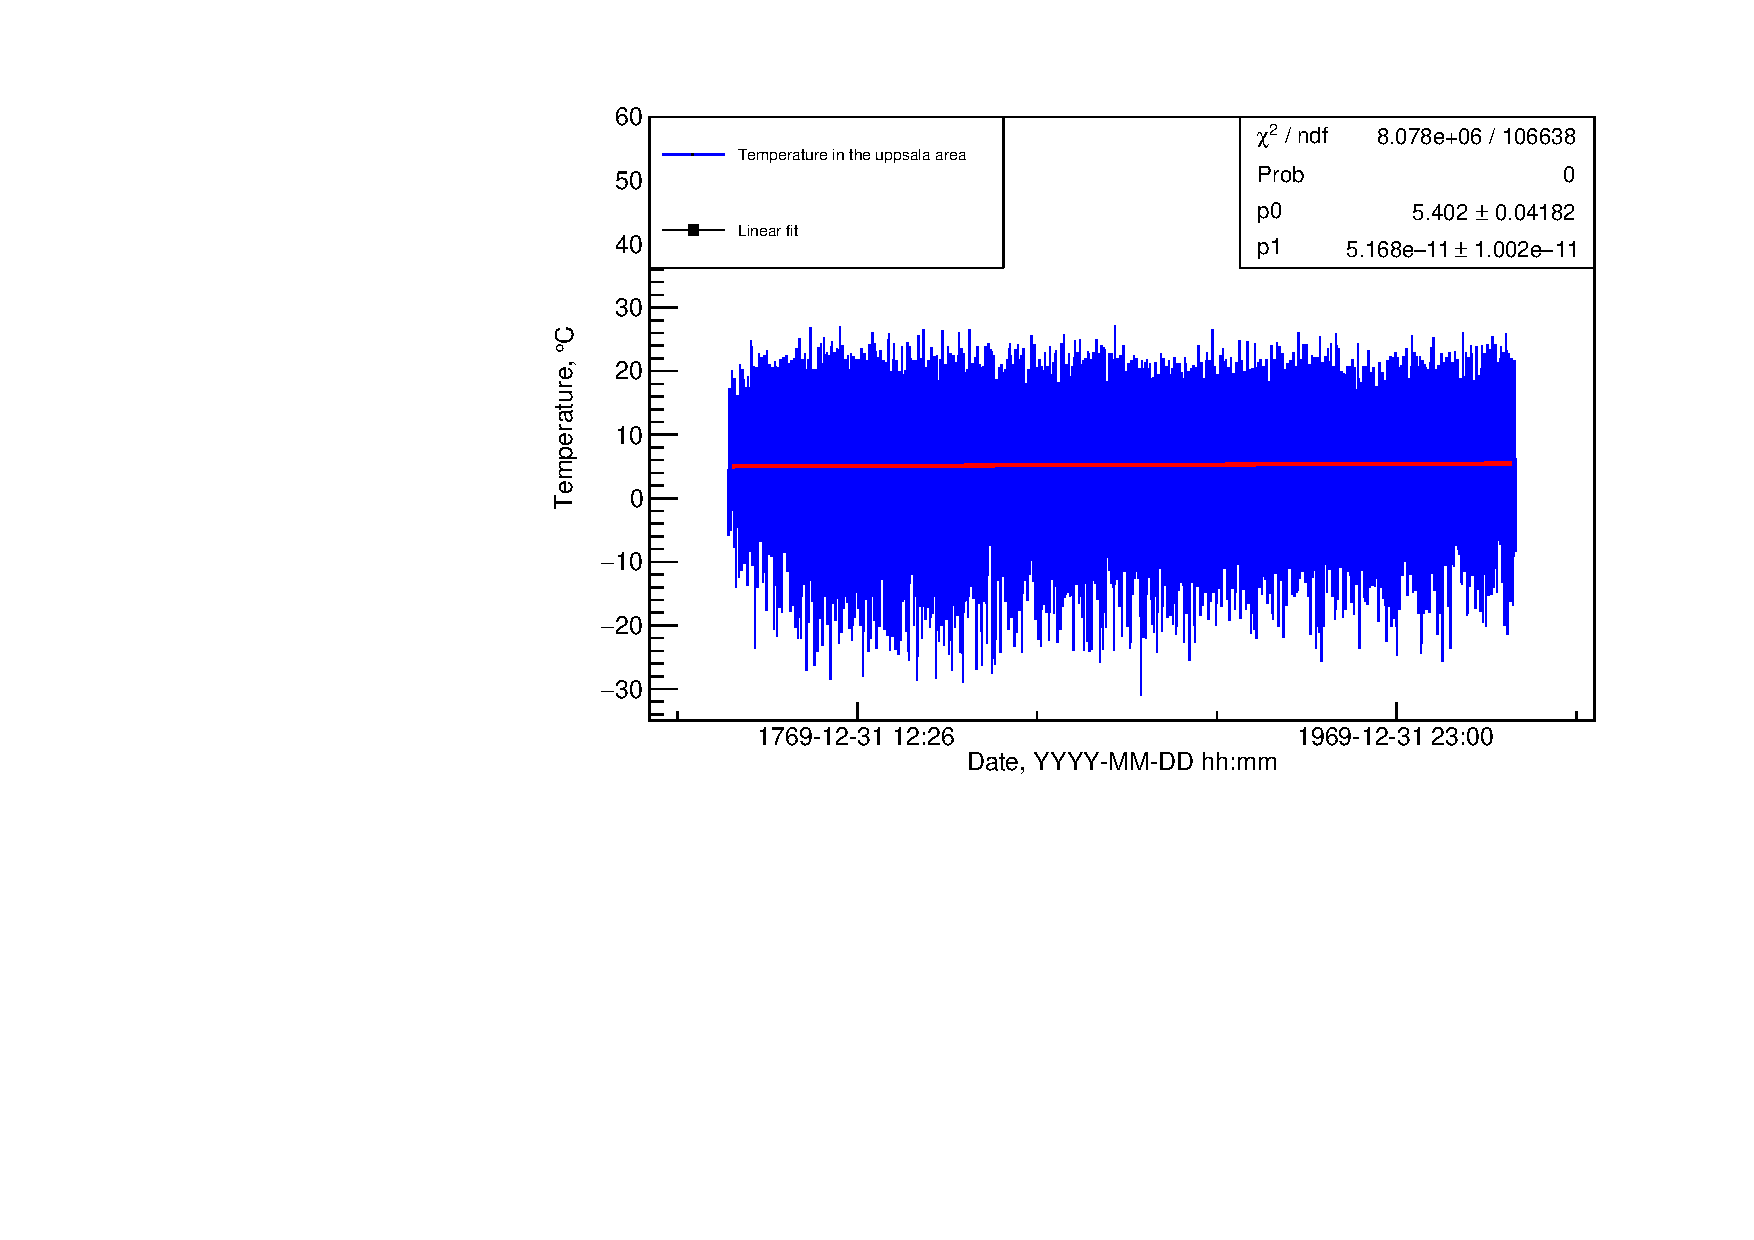
\includegraphics[width=0.8\linewidth]{temperature_uppsala.pdf}}\\
    \subfloat{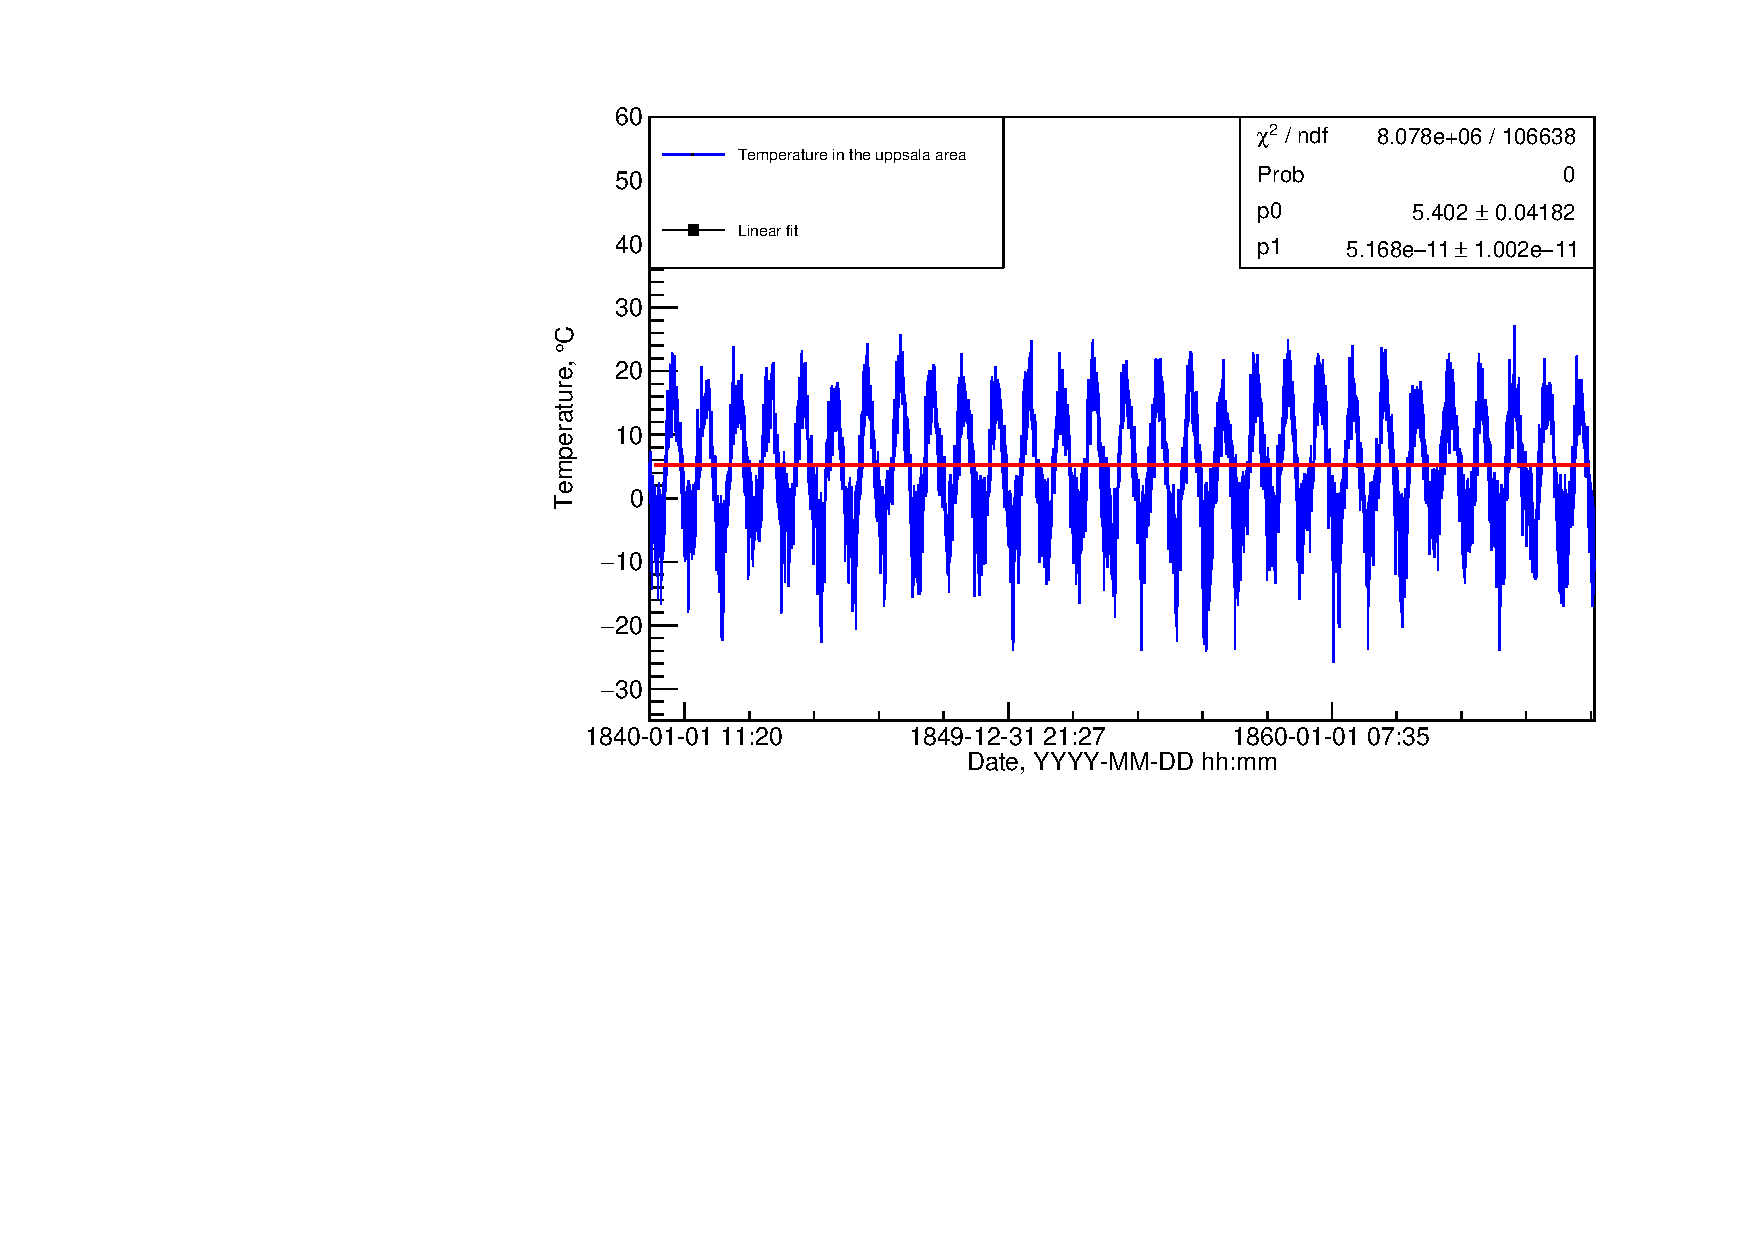
\includegraphics[width=0.8\linewidth]{temperature_uppsala_zoomed.pdf}}
    \caption{An example of output of \texttt{getTemperature} function. Top panel:
    the full range of data. Bottom panel: a reduced sample of 10\% of the data,
    from the middle of the data set.}
    \label{fig:getTemperature}
\end{figure}



\section{Results}



Figure \ref{fig:everyDay} In the everyDay and LattDiff section shows what we expect, there is a clear region for each of the seasons 

\begin{figure}[h!]
    \centering
    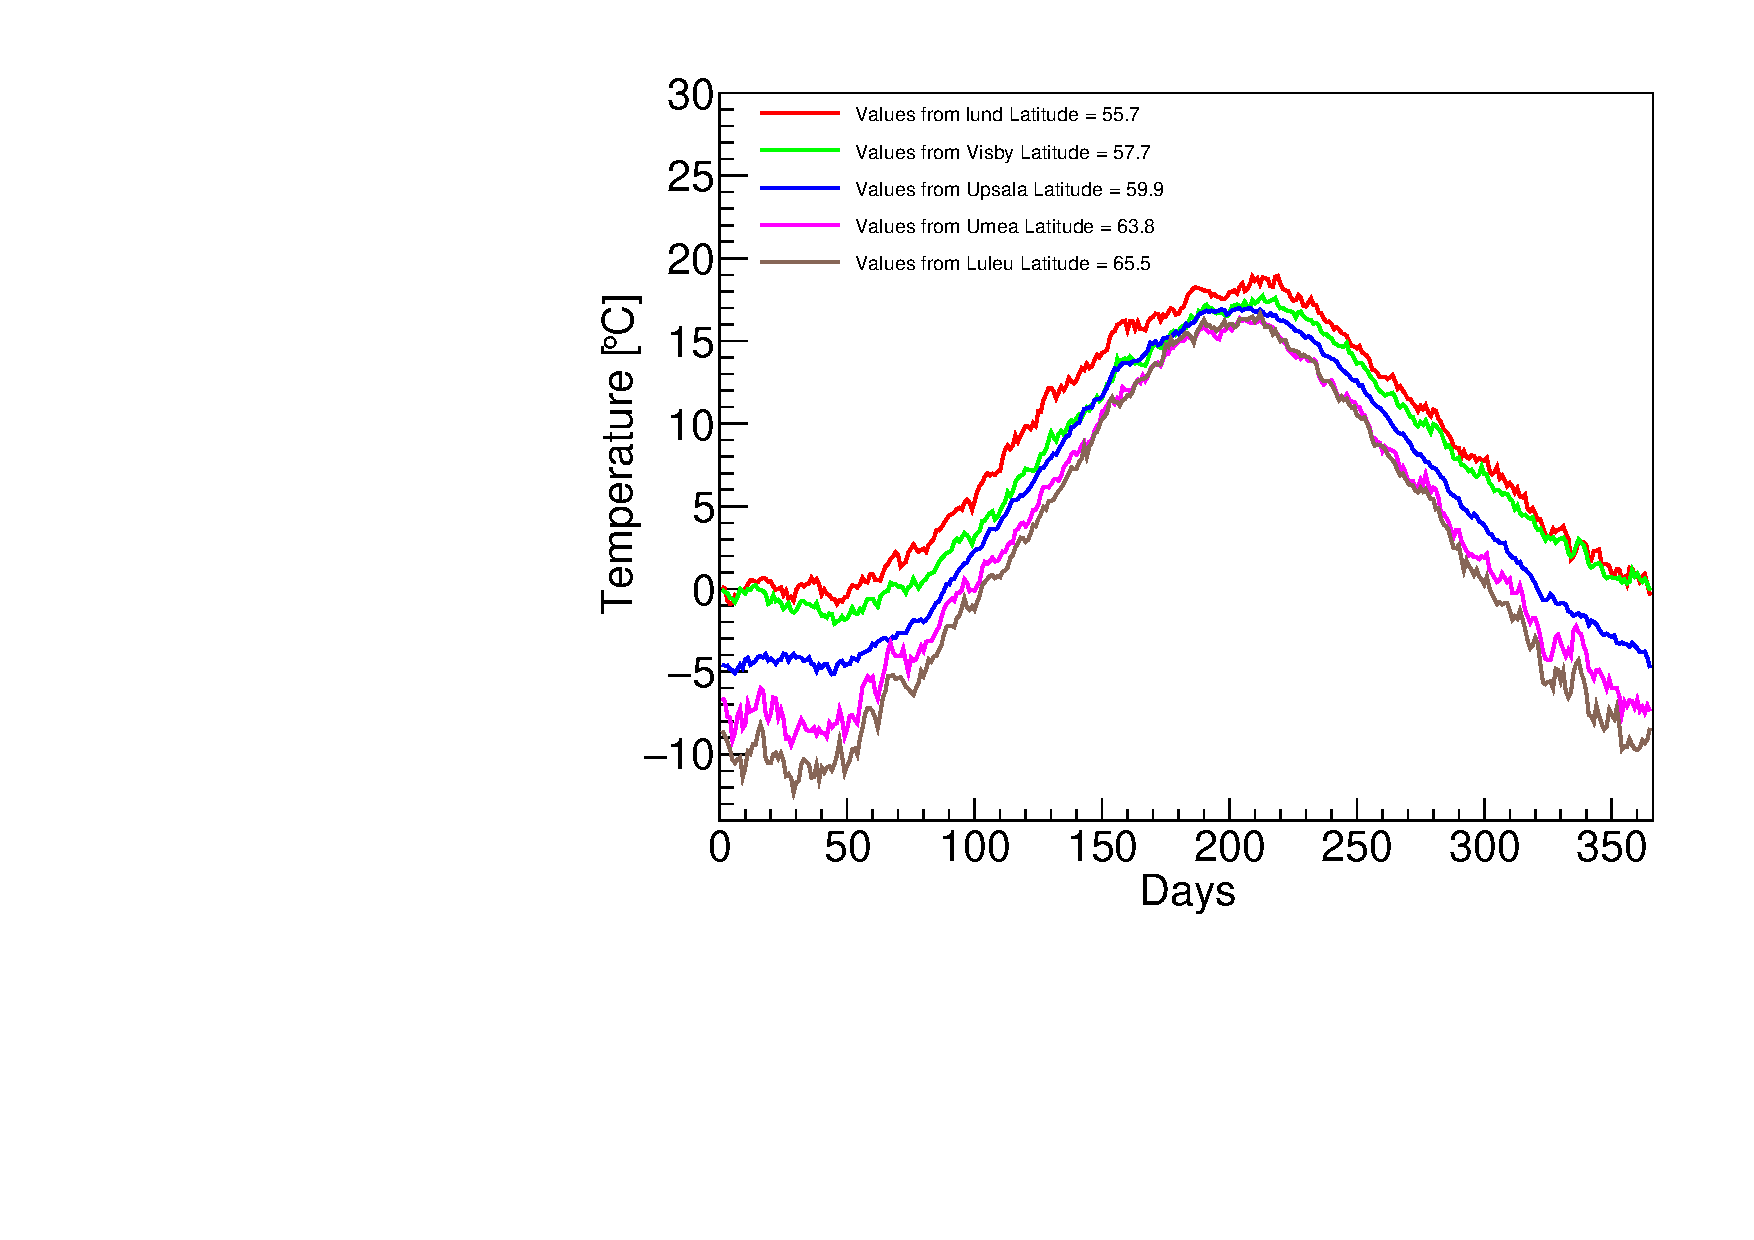
\includegraphics[scale = 0.7]{every_day_graph_multiple_locations_just_means.pdf}
    \caption{Plot produced by the LattDiff function showing only the mean}
    \label{fig:LattDiff_no}
\end{figure}

From Figure \ref{fig:LattDiff_no} we see that as expected the overall temperature tends to increase as the latitude decreases.


The analysis of the data as to the average temperature and increase of temperature 
overtime is presented in Table~\ref{tab:tempr_trend}. It was found that the data for first 10 years of
measurements for Falun location was corrupted (Figure \ref{fig:falund}), this data was
removed from the analysis.

\begin{figure}
    \centering
    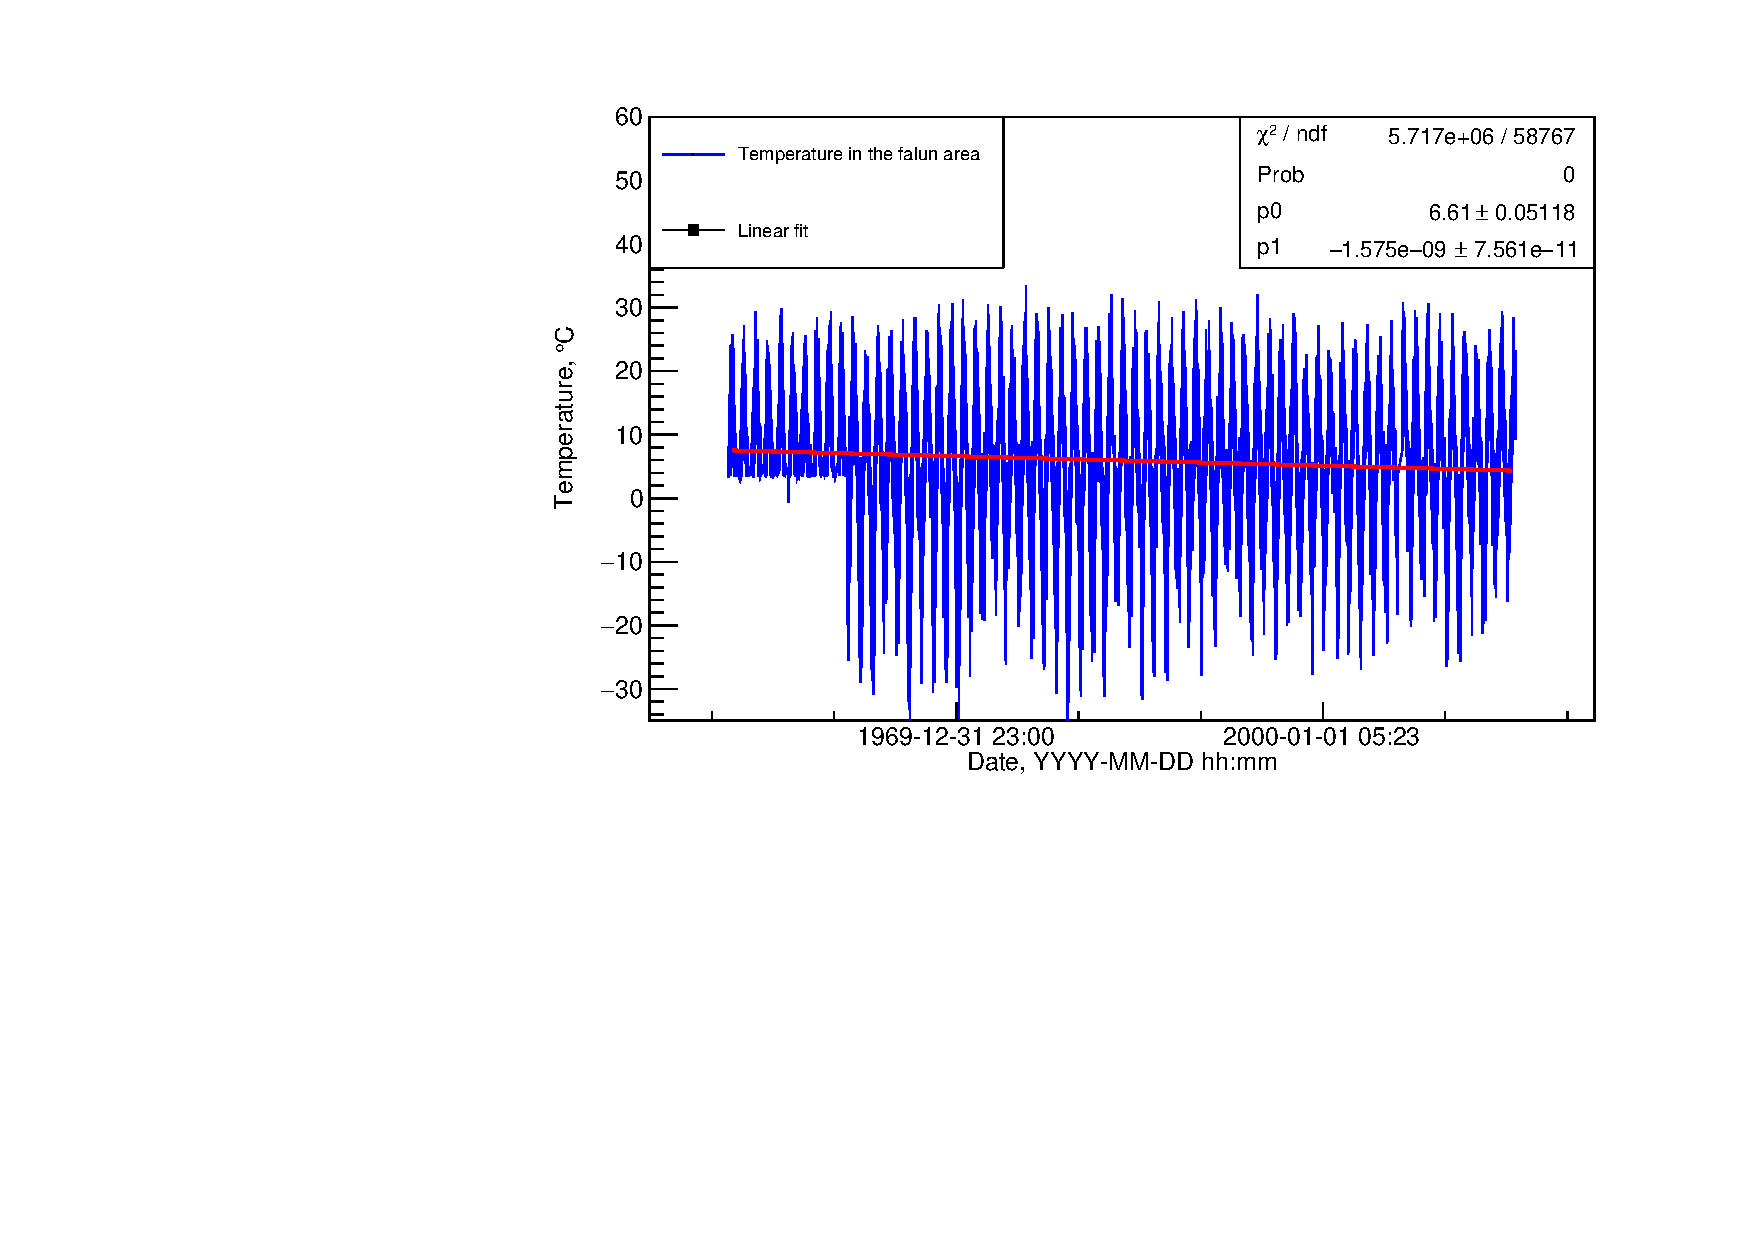
\includegraphics[width=0.8\linewidth]{temperature_falun_corrupted.pdf}
    \caption{The data set for the Falund location, note the data corruption for 
    the first 10 years. This corrupted data was excluded from the analysis.}
    \label{fig:falund}
\end{figure}

\begin{table}
    \centering
    \begin{tabular}{lrr}
Location& Average Temperature, $^\circ$C& Change of average temperature, $^\circ$C/year\\
\hline
Boras&    $6.59\pm0.05$&                  $0.015\pm0.002$\\
Falsterbo&$8.13\pm0.02$&                  $0.030\pm0.001$\\
Falun&    $4.85\pm0.08$&                  $0.020\pm0.003$\\
Karlstad& $6.31\pm0.02$&                  $0.002\pm0.001$\\
Lulea&    $1.91\pm0.02$&                  $0.024\pm0.001$\\
Lund&     $8.36\pm0.05$&                  $0.011\pm0.002$\\
Soderarm& $5.61\pm0.02$&                  $0.038\pm0.001$\\
Umea&     $2.42\pm0.02$&                  $0.041\pm0.001$\\
Uppsala&  $5.40\pm0.04$&                  $0.002\pm0.000$\\
Visby&    $6.93\pm0.01$&                  $0.022\pm0.001$\\
\hline
    \end{tabular}
    \caption{Average temperature and change of average temperature over time for the selected 10 data sets.
    Details in the text.}
    \label{tab:tempr_trend}
\end{table}

From the results presented in Table \ref{tab:tempr_trend} one can notice, that for each data sample, a positive
change of average temperature is observed. This change is especially noticeable for the data gathered in 20 century.
This fact could indicate a connection between the temperature and increase of power consumption by society in
the recent 100 years. Another noticeable fact is that the change of average temperature is the highest in the 
locations with lowest temperature in the analysed data.

\end{document}
